\section{Manual de usuario}\label{Manual usuario}

Para el correcto uso de la aplicación, el conjunto de acciones que se pueden realizar en dicho programa serán definidas a continuación. También, la distribución de las secciones de la interfaz junto a su explicación y funcionalidad.\bigskip

Cuando se ejecute el programa por primera vez en la pantalla se debe mostrar la siguiente interfaz de usuario:

\begin{figure}[!h]
    \centering
    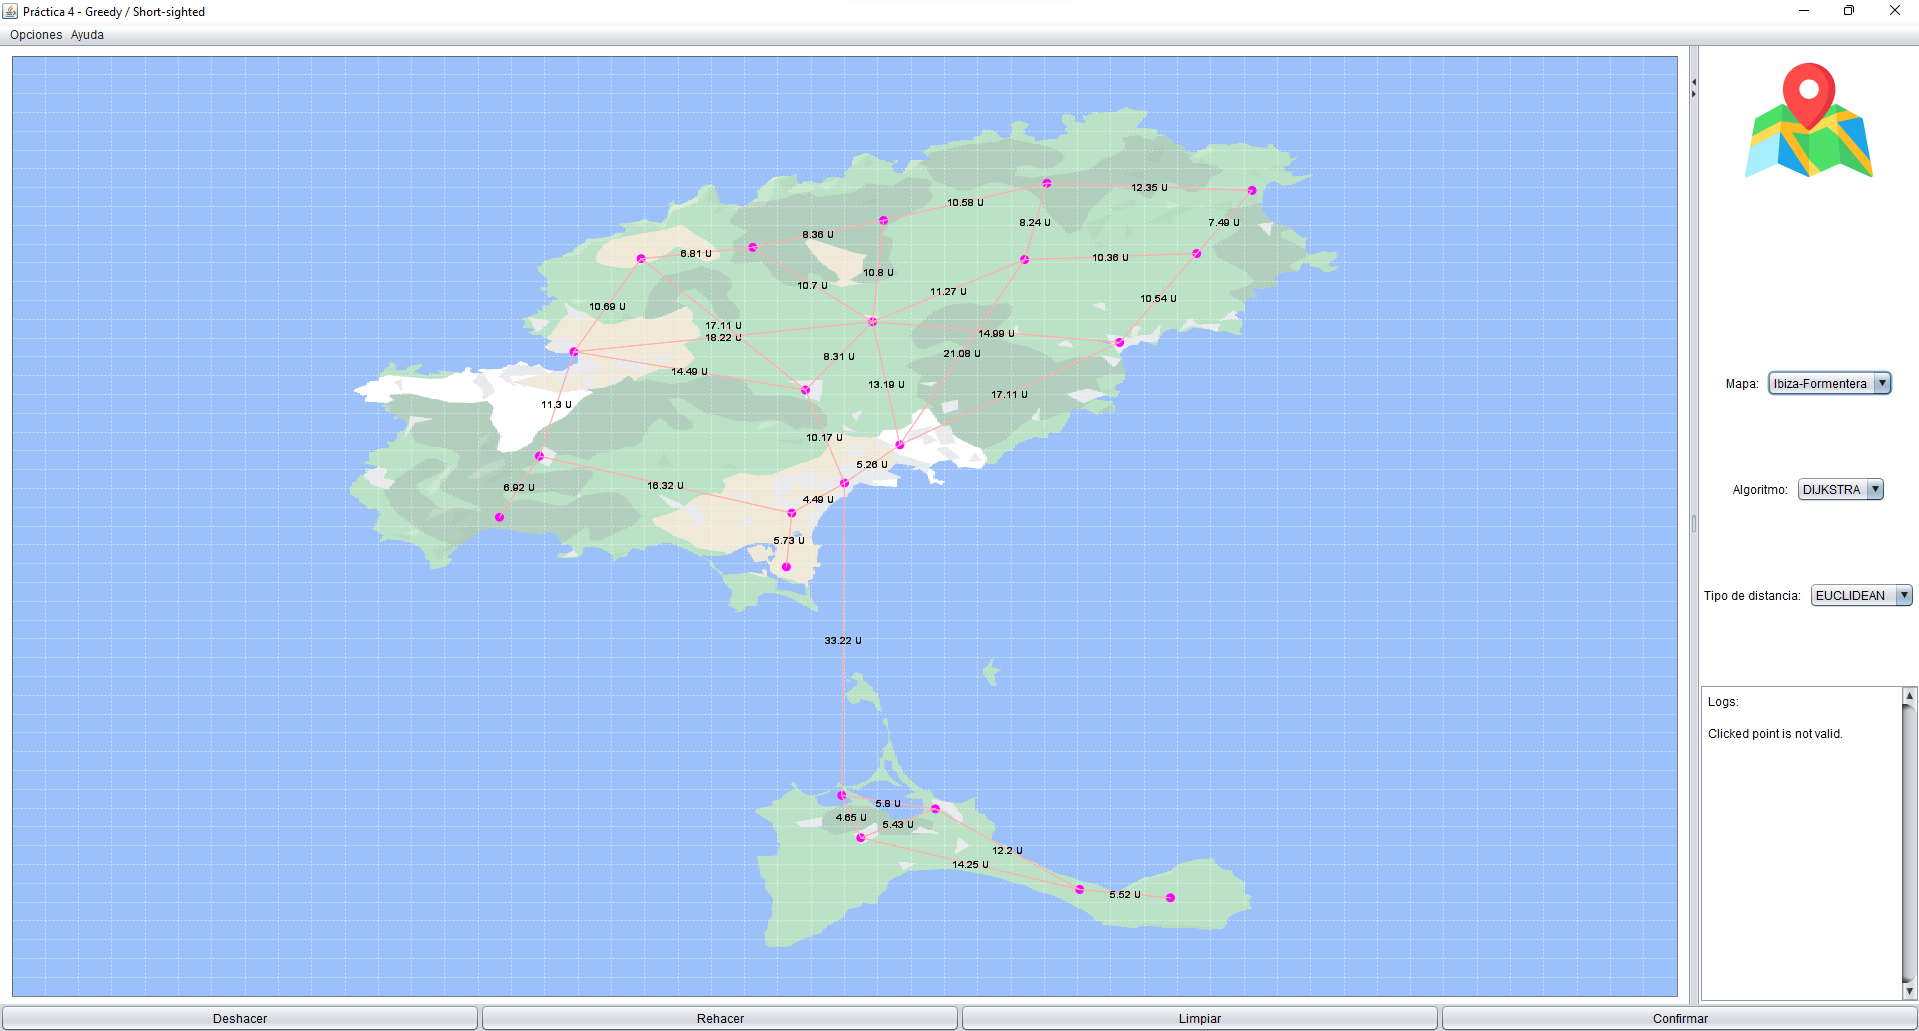
\includegraphics[width=\linewidth]{Usage/img/GUI.png}
    \caption{Interfaz de usuario.}
    \label{fig:User_interface}
\end{figure}

\subsection{Menu}\label{Manual usuario, Header}

El menú de la aplicación se trata de la barra que se sitúa debajo del marco superior de la ventana. En esta se puede encontrar un conjunto de opciones para que el usuario pueda interactuar con la aplicación, modificar y analizar el comportamiento de esta. En concreto, se encuentran las opciones de \say{Opciones} y \say{Ayuda}.\bigskip

En la primera se sitúan las acciones para salir del programa y para borrar y/o resetear datos e iniciar las ventanas de estadísticas explicadas anteriormente en los apartados \ref{Stats JVM} y \ref{Stats Algt}.\bigskip

En la otra opción se encuentra un menú desplegable con un manual de usuario con la explicación del funcionamiento de la aplicación.

\subsection{Main}

El \say{Main} es el bloque principal de la vista, donde se representará el mapa con las poblaciones, aquí el usuario podrá seleccionar los puntos/poblaciones para encontrar el camino mínimo. El usuario deberá clicar de manera precisa en el punto, debido a que éste tiene un radio de detección del ratón determinado. De esta manera, al clicar en el mapa, no se seleccionará ningún punto de manera errónea. No podrá clicar dos veces sobre el mismo punto. \bigskip

\subsection{Sidebar}\label{Sidebar}

El \say{Sidebar} contiene un conjunto de opciones para modificar los datos y el modo de ejecución de la aplicación. A continuación, se explicará cada una de estas opciones y su función.\bigskip

En primer lugar, se encuentra la opción para seleccionar el \say{Mapa}. En esta, se puede escoger el mapa que queremos representar. En esta práctica, se han implementado los siguientes mapas: \bigskip

\begin{itemize}
    \item Ibiza-Formentera
    \item Ibiza
    \item Formentera
\end{itemize}
\bigskip

En segundo lugar, se halla la opción para elegir el \say{Algoritmo}. En esta opción, se tiene la opción cambiar el algoritmo a aplicar sobre los puntos seleccionados. De manera que el resultado podría cambiar dependiendo del algoritmo ejecutado. Los algoritmos implementados son:\bigskip

\begin{itemize}
    \item Dijkstra
    \item Greedy 
\end{itemize}
\bigskip

En tercer lugar, se encuentra el \say{Tipo de distancia}. Esta opción permite definir una heurística para calcular la distancia. Las heurísticas implementadas son:\bigskip

\begin{itemize}
    \item Euclidean
    \item Manhattan 
    \item Chebyshev
    \item Cosine
    \item Minkowski
    \item Haversine
\end{itemize}
\bigskip

En tercer lugar, se encuentra una ventana de \say{logs}. En esta ventana el usuario tendrá una noción de lo que está ocurriendo en el programa, indicando los puntos seleccionados y si se ha seleccionado fuera del mapa. \bigskip

\subsection{Footer}\label{Footer}

En la sección \say{Footer}, se hallan cuatro botones para interactuar con los puntos seleccionados sobre el mapa.
En primer lugar, empezando por la izquierda de la interfaz, tenemos el botón \say{Deshacer}. Cuando el botón sea pulsado, el último punto añadido al mapa será borrado.\bigskip

En segundo lugar, tenemos el botón \say{Rehacer}. Cuando se pulse este botón, el último punto eliminado será añadido sobre el mapa de nuevo. En el momento en el que el usuario añada un nuevo punto después de haber pulsado \say{Deshacer}, no podrá rehacer ningún punto.\bigskip 

En tercer lugar, se encuentra el botón \say{Limpiar}, con este botón desaparecerán todos los elementos añadidos sobre el mapa tras haber iniciado el programa y volverá a su estado inicial. Este botón es útil para borrar todos los puntos seleccionados o la solución del camino.\bigskip

Por último, se halla el botón \say{Confirmar}. Este botón envía al Controlador los puntos seleccionados y ejecuta el algoritmo, una vez ejecutado se representará el camino en el mapa, con una línea de color rojo. 

\subsection{Ejemplo ejecución}

Al iniciar la aplicación se mostrará una interfaz como la expuesta en la imagen \ref{fig:User_interface}. Para poder iniciar la ejecución del algoritmo, es necesario seleccionar dos o más puntos sobre el mapa, en el caso de equivocarse podrá \say{Deshacer} y \say{Rehacer} los puntos. Además, de poder borrarlos todos con el botón \say{Limpiar}. Al clicar en \say{Confirmar}, si hay dos o más puntos en el mapa, se ejecutará el algoritmo y se pintará sobre el mapa el camino mínimo entre los puntos seleccionados. A continuación, la siguiente imagen, muestra un ejemplo de la interfaz en mitad de la ejecución:

\begin{figure}[!h]
    \centering
    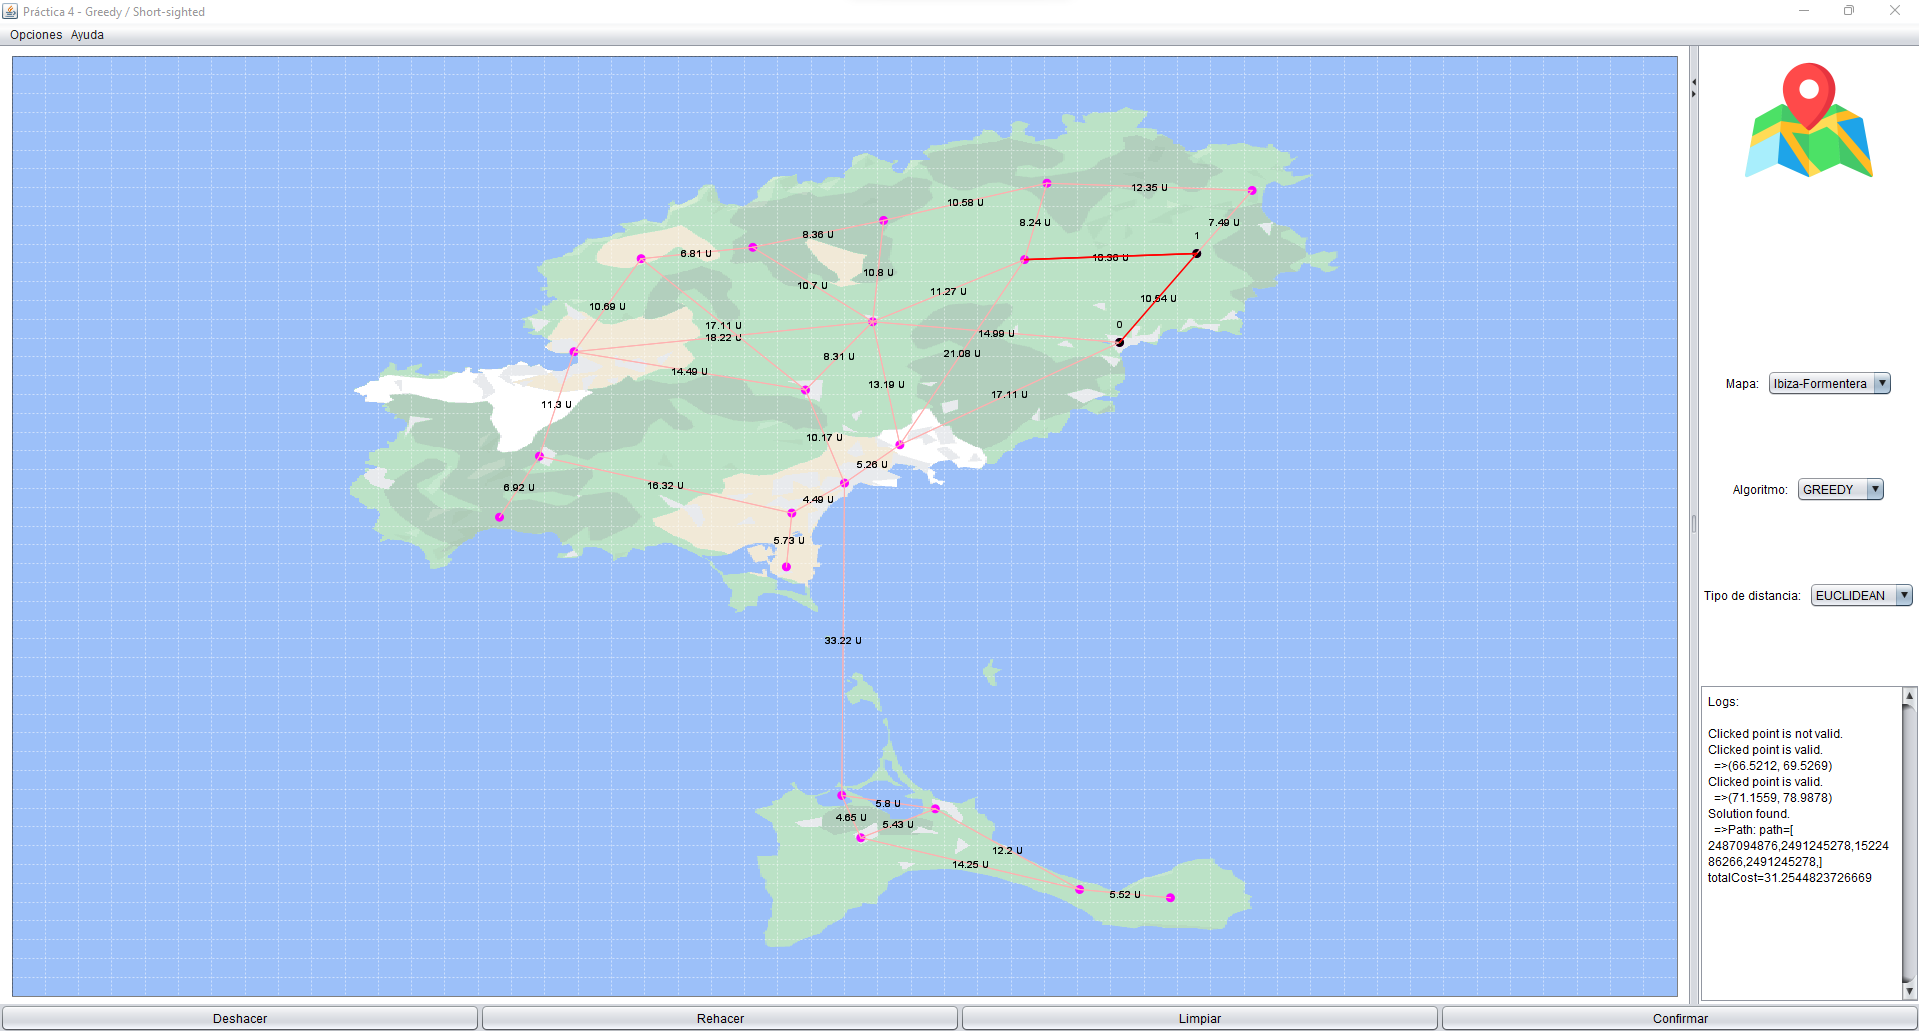
\includegraphics[width=\linewidth]{Usage/img/ejecucion.png}
    \caption{Interfaz de usuario en ejecución.}
    \label{fig:Ejemplo ejecución}
\end{figure}

A partir de aquí, el usuario puede reiniciar la ejecución para ejecutar nuevamente el algoritmo, borrar las soluciones obtenidas, ejecutar otros algoritmos, cambiar el tipo de distancia, cambiar el mapa y ver estadísticas de la ejecución, ver apartados \ref{Stats JVM} y \ref{Stats Algt}.
